
%%%%%%%%%%%%%%%%%%%%%%%%%%%%%%%%%%%%%%%%%%%%%%%%%%%%%%%%%%%%%%%%%%%%%%%%%%%%%%%%
%%%%%%%%%%%%%%%%%%%%%%%%%%%%%%%%%%%%%%%%%%%%%%%%%%%%%%%%%%%%%%%%%%%%%%%%%%%%%%%%
\newpage

In what follows the tolerance is set to $10^{-7}$ and a relaxation factor of 3/4. 
Results are obtained with {\tt script\_onset}.
We find that the critical Rayleigh number is between 775 and 780.
Also, results are not very sensitive to resolution.
When $\Ranb$ is close to its critical value the scheme requires a lot of iterations
as it very slowly converges.

\subsection*{Onset of convection}

\begin{center}
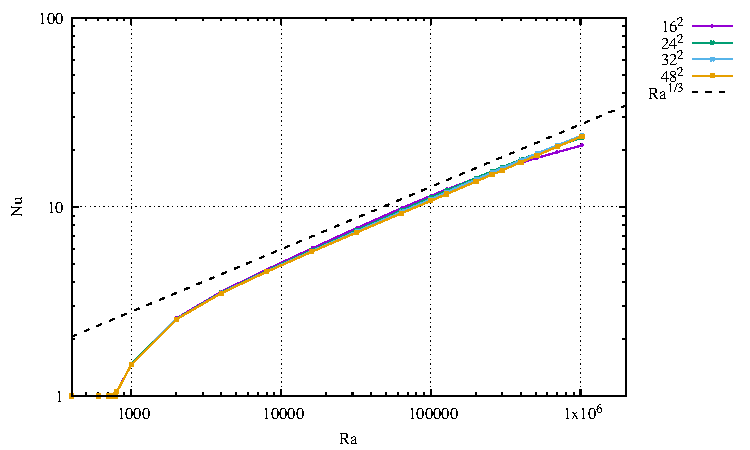
\includegraphics[width=8cm]{python_codes/md/results_new/onset}
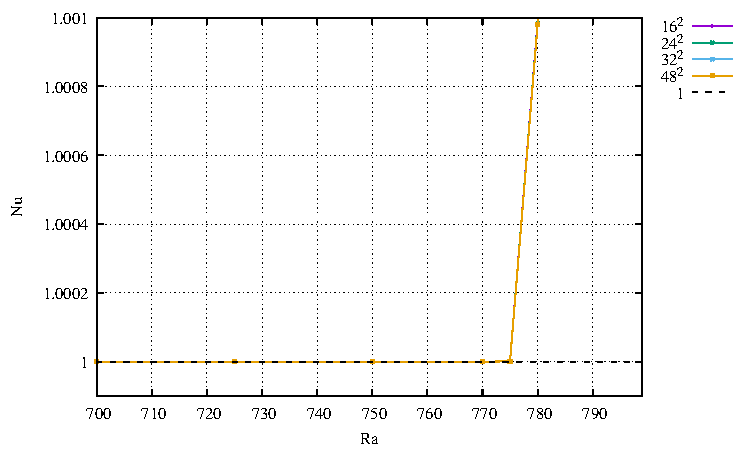
\includegraphics[width=8cm]{python_codes/md/results_new/onset_zoom}
\end{center}

Because the onset of convection (controlled by the critical Rayleigh 
number seems to be between 770 and 780 we can run a simple test 
of about 10 iterations only (no steady state is reached) and look at 
the evolution of the $\upnu_{rms}$. If it decreases then convection is dying out
and we are in a purely conductive regime. 
It it increases then convection is going to occur.
\begin{center}
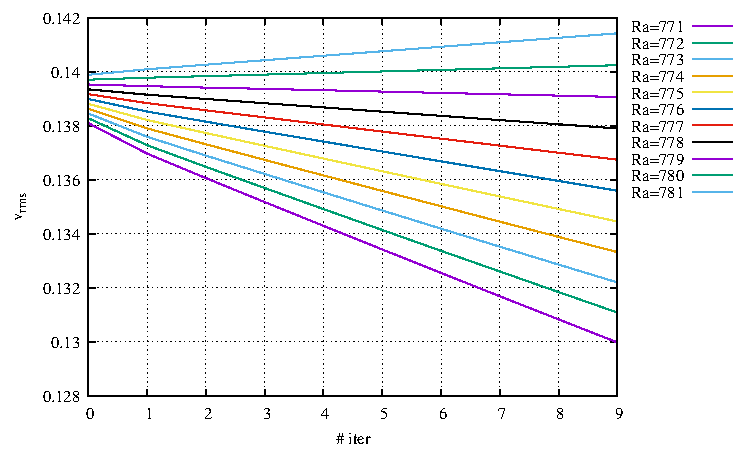
\includegraphics[width=8cm]{python_codes/md/results_onset2/vrms}
\end{center}

\newpage
\subsection*{Temperature profiles}

\begin{center}
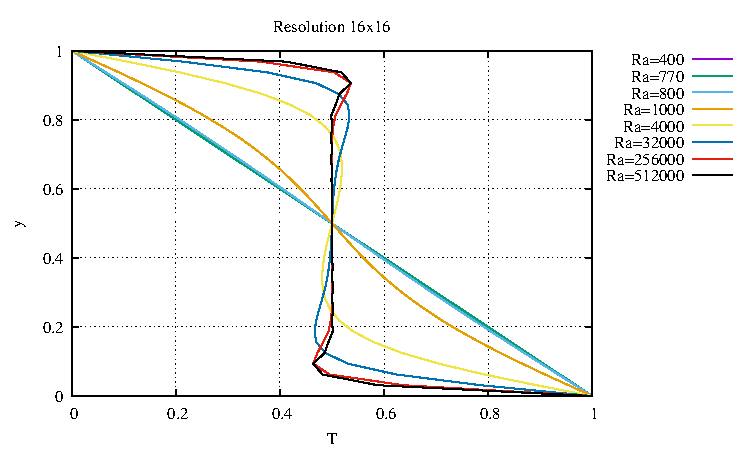
\includegraphics[width=8cm]{python_codes/md/results_new/profile_16x16}
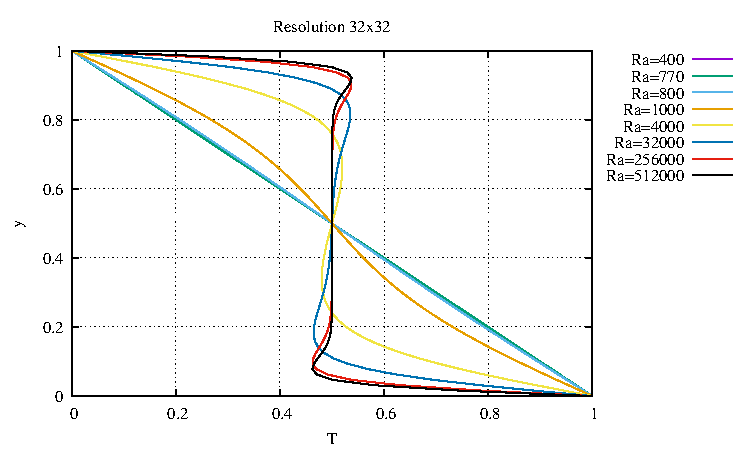
\includegraphics[width=8cm]{python_codes/md/results_new/profile_32x32}\\
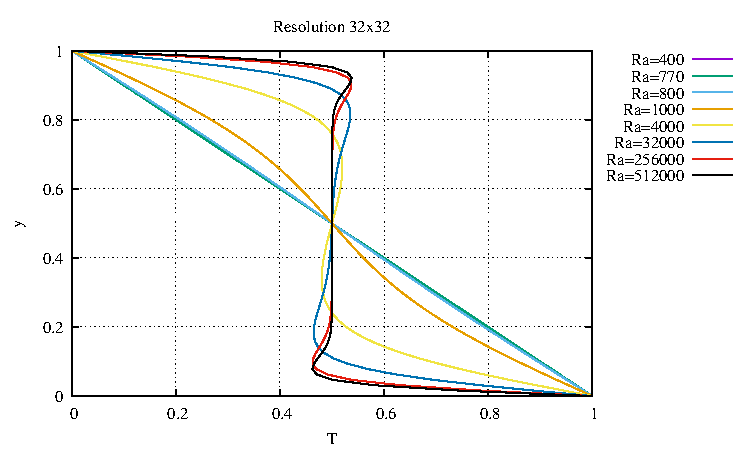
\includegraphics[width=8cm]{python_codes/md/results_new/profile_32x32}
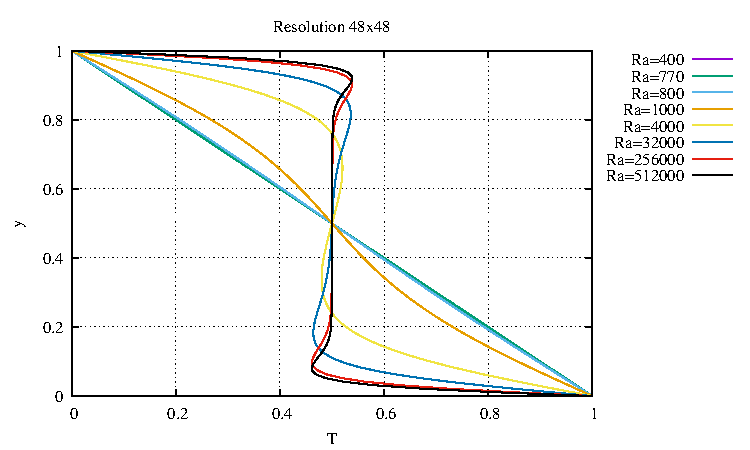
\includegraphics[width=8cm]{python_codes/md/results_new/profile_48x48}
\end{center}

\newpage
\subsection*{Nusselt number}

Results shown for Nusselt number between 700 and 800.

\begin{center}
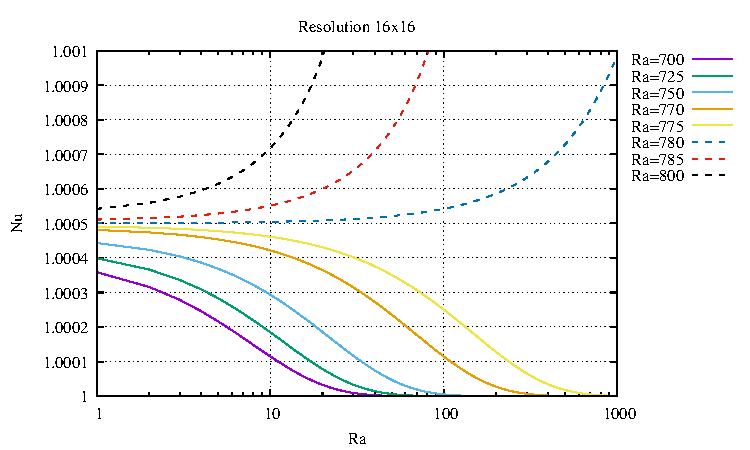
\includegraphics[width=8cm]{python_codes/md/results_new/Nu_16x16}
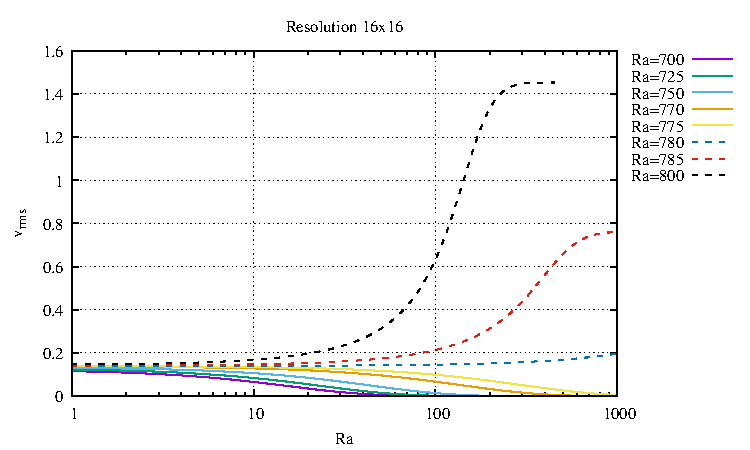
\includegraphics[width=8cm]{python_codes/md/results_new/vrms_16x16}\\
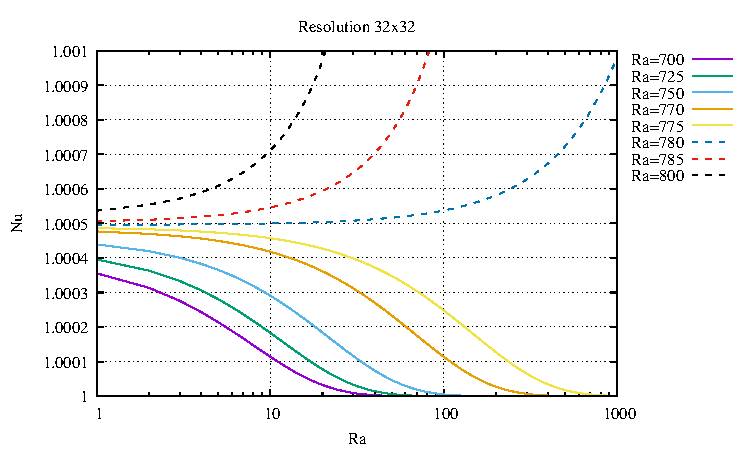
\includegraphics[width=8cm]{python_codes/md/results_new/Nu_32x32}
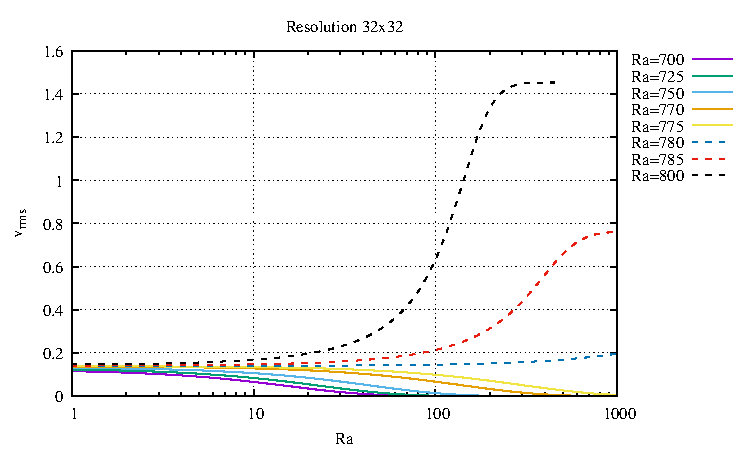
\includegraphics[width=8cm]{python_codes/md/results_new/vrms_32x32}\\
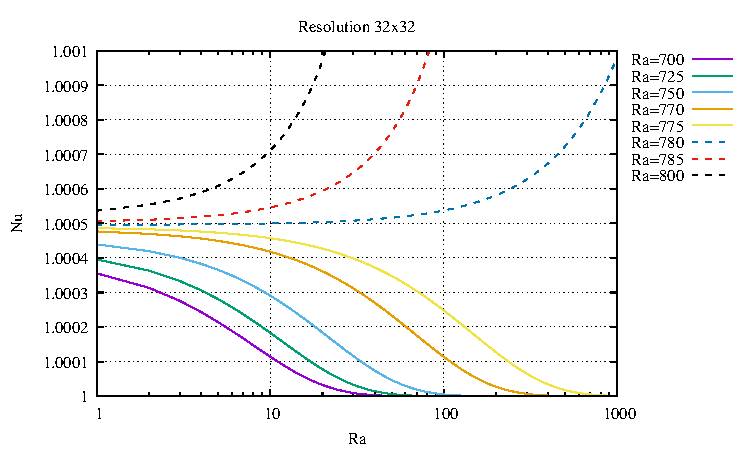
\includegraphics[width=8cm]{python_codes/md/results_new/Nu_32x32}
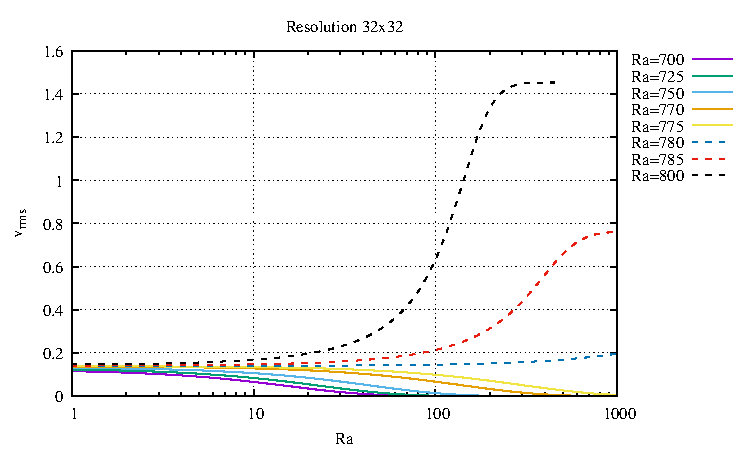
\includegraphics[width=8cm]{python_codes/md/results_new/vrms_32x32}\\
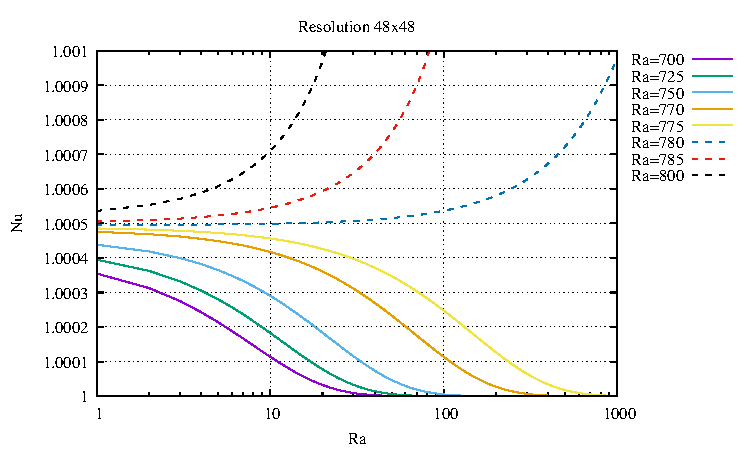
\includegraphics[width=8cm]{python_codes/md/results_new/Nu_48x48}
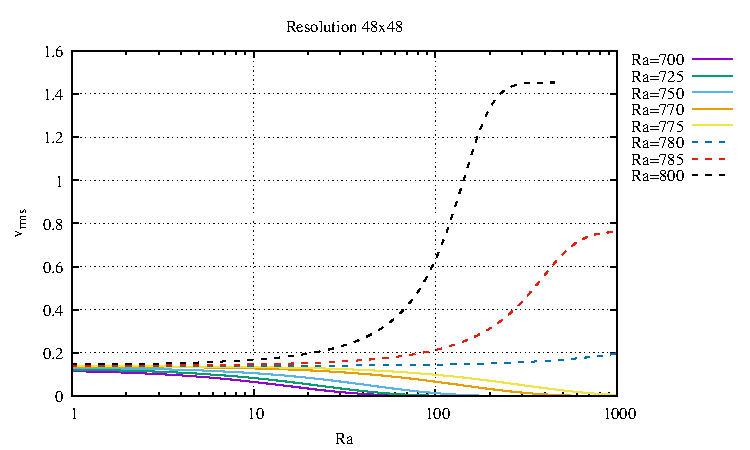
\includegraphics[width=8cm]{python_codes/md/results_new/vrms_48x48}
\end{center}


\newpage
\subsection*{convergence}
\begin{center}
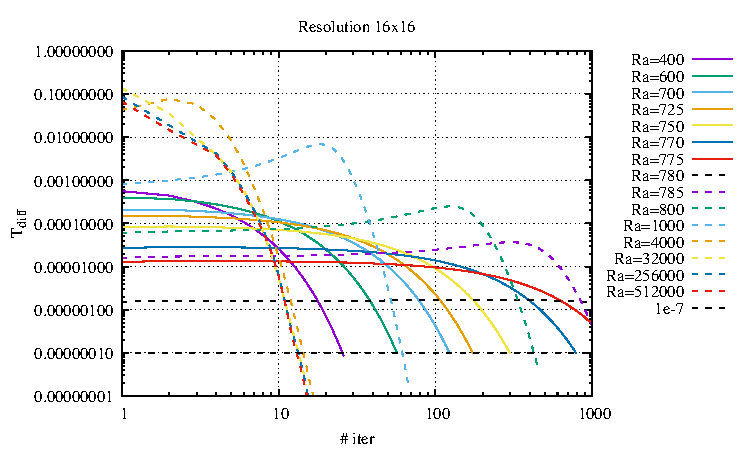
\includegraphics[width=8cm]{python_codes/md/results_new/conv_16x16_T.pdf}
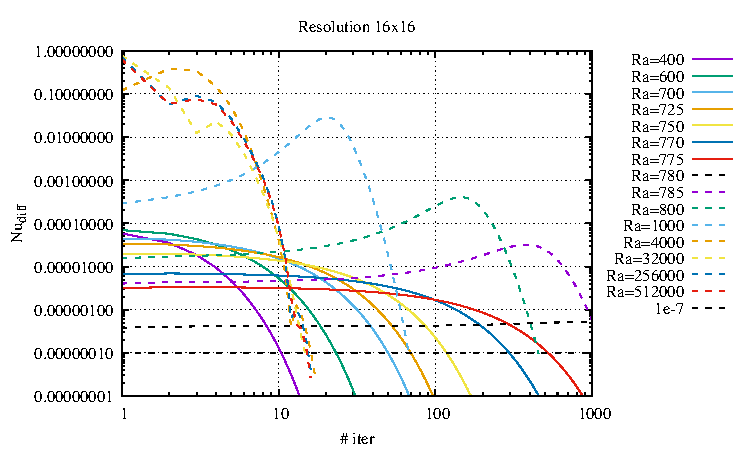
\includegraphics[width=8cm]{python_codes/md/results_new/conv_16x16_Nu.pdf}\\
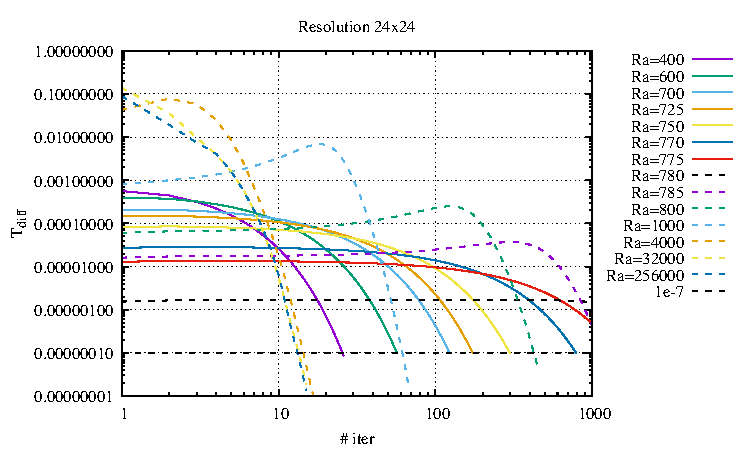
\includegraphics[width=8cm]{python_codes/md/results_new/conv_24x24_T.pdf}
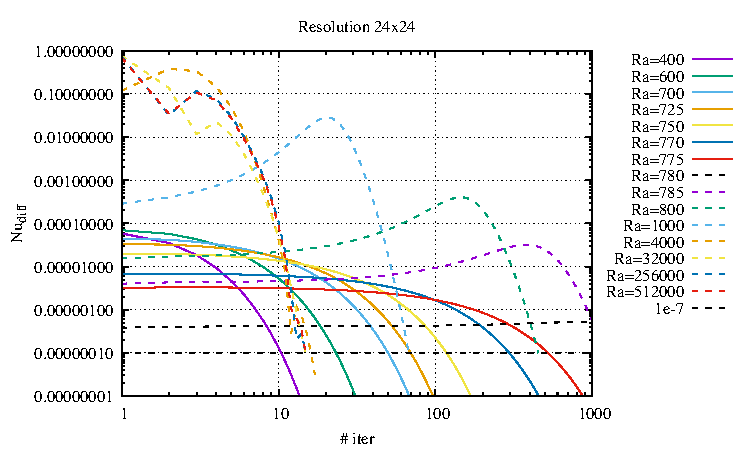
\includegraphics[width=8cm]{python_codes/md/results_new/conv_24x24_Nu.pdf}\\
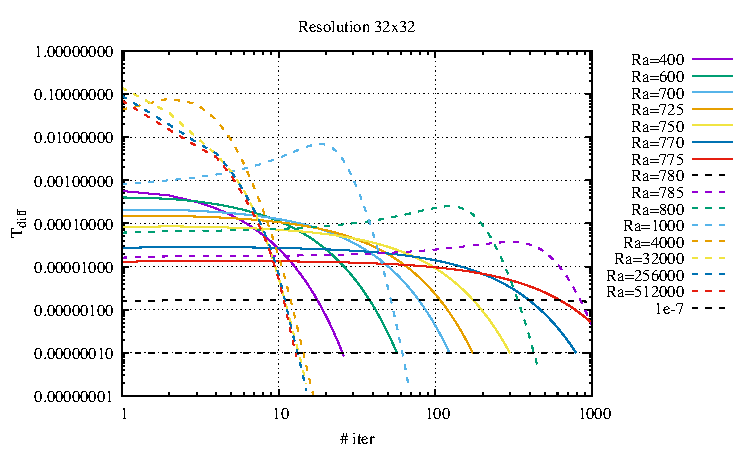
\includegraphics[width=8cm]{python_codes/md/results_new/conv_32x32_T.pdf}
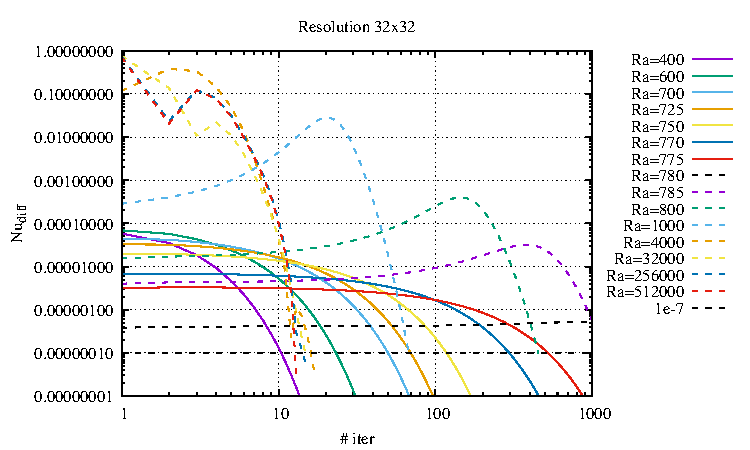
\includegraphics[width=8cm]{python_codes/md/results_new/conv_32x32_Nu.pdf}\\
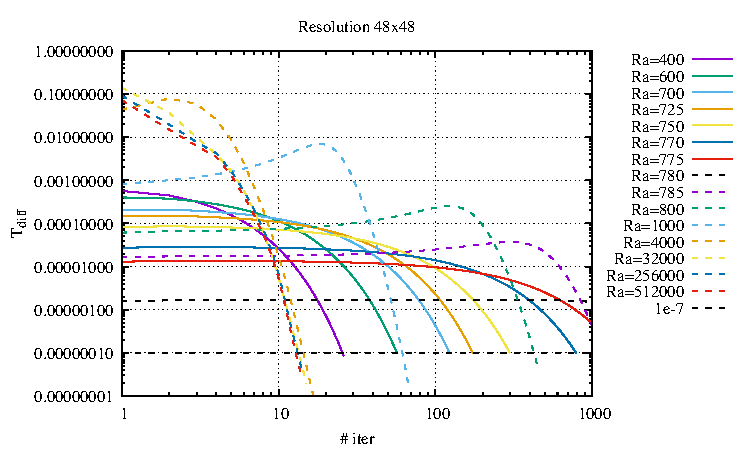
\includegraphics[width=8cm]{python_codes/md/results_new/conv_48x48_T.pdf}
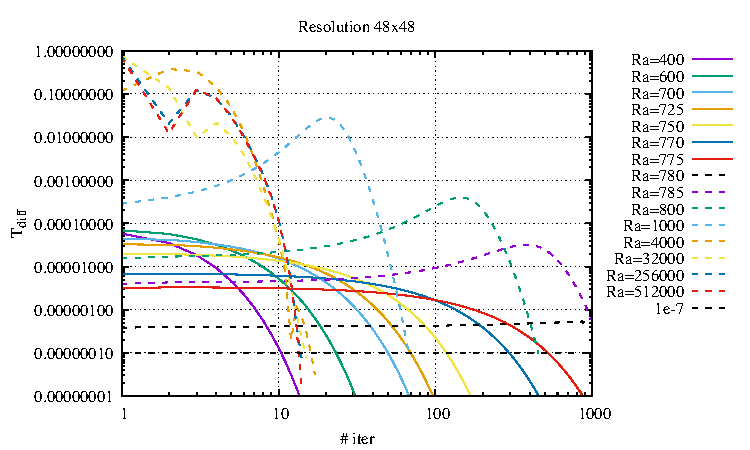
\includegraphics[width=8cm]{python_codes/md/results_new/conv_48x48_Nu.pdf}
{\captionfont } 
\end{center}

\newpage
\subsection*{Steady state resolution tests}

The following results are obtained with {\tt script\_steadystate}.
Values are those from \textcite{blbc89}.

\begin{center}
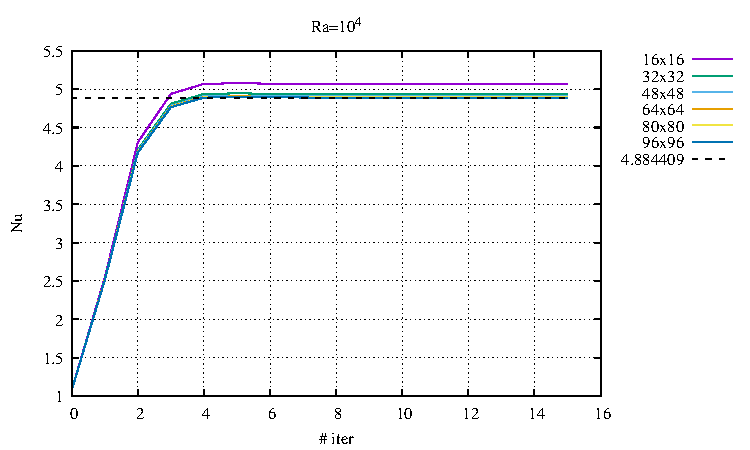
\includegraphics[width=8cm]{python_codes/md/results_ss/Nu_Ra1e4.pdf}
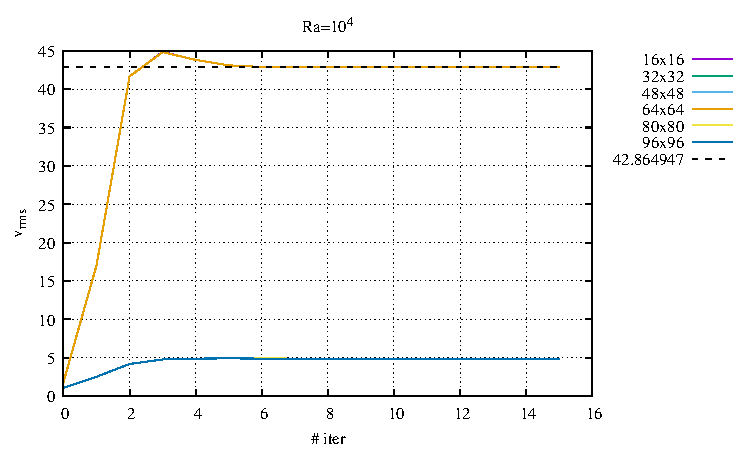
\includegraphics[width=8cm]{python_codes/md/results_ss/vrms_Ra1e4.pdf}\\
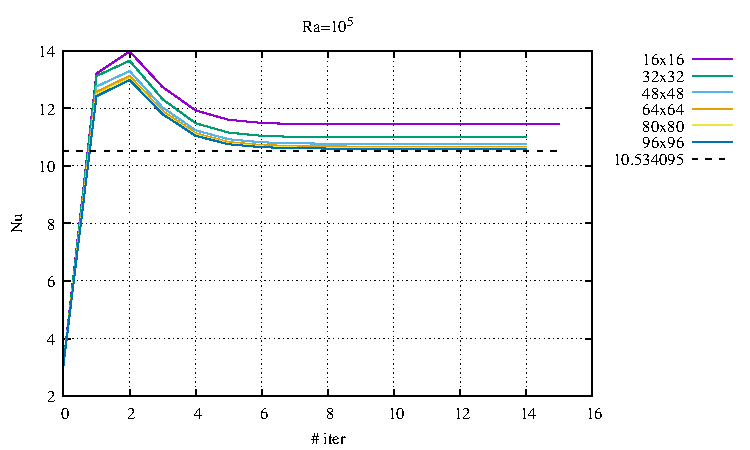
\includegraphics[width=8cm]{python_codes/md/results_ss/Nu_Ra1e5.pdf}
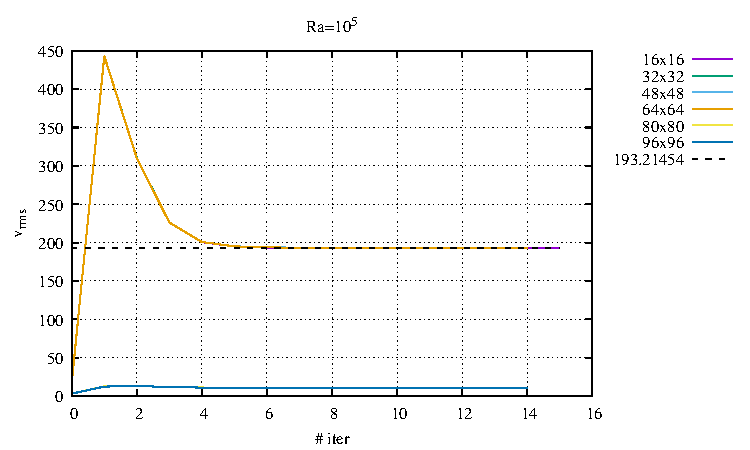
\includegraphics[width=8cm]{python_codes/md/results_ss/vrms_Ra1e5.pdf}\\
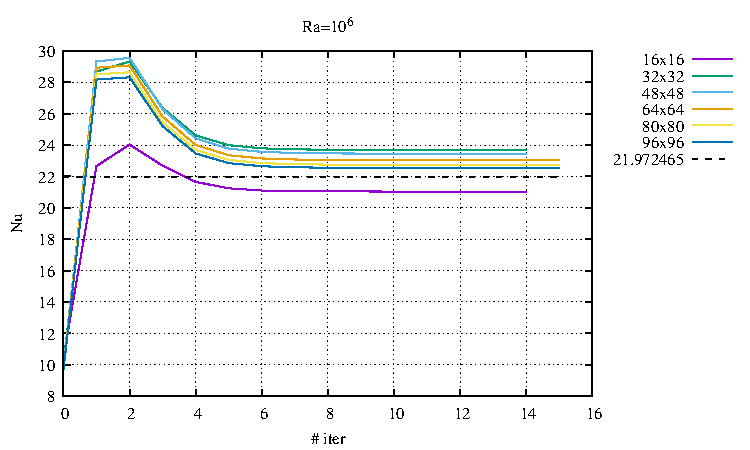
\includegraphics[width=8cm]{python_codes/md/results_ss/Nu_Ra1e6.pdf}
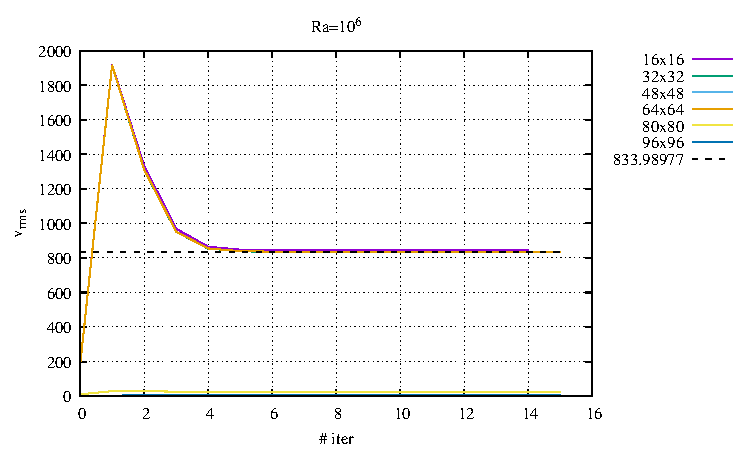
\includegraphics[width=8cm]{python_codes/md/results_ss/vrms_Ra1e6.pdf}
\end{center}




